\documentclass{IEEEtran}
\usepackage{filecontents}
\usepackage{lipsum}
\usepackage[utf8]{inputenc}
\usepackage{graphicx} % for image
\usepackage{color} % for image (?)
\usepackage{amsmath}
\usepackage{verbatim}
\usepackage{tikz} %to draw the graphs
\usetikzlibrary{shapes.gates.logic.US,trees,positioning,arrows}
% correct bad hyphenation here
\hyphenation{op-tical net-works semi-conduc-tor}

\begin{document}

\title{SSA - Título Provisório:\\Otimização do perfil de tensão em Linhas de Distribuição de Energia por Injeção de Potência Reativa}


\author{Luiz~Le~Roy - ~\IEEEmembership{PUC Minas}
        % <-this % stops a space
\thanks{Texto iniciado em 4 de abril de 2014.}}

% The paper headers
\markboth{IEEE Transaction on \LaTeX\,~Vol.~X, No.~Y, Abril~2014}%
{Shell \MakeLowercase{\textit{et al.}}: Bare Demo of IEEEtran.cls for Journals}

% make the title area
\maketitle

%%%\begin{abstract}

%%%\end{abstract}

\begin{IEEEkeywords}
ORP \textit{(Optimal Reactive Power)}, OCP \textit{(Optimal Capacitor Placement)}, DSSE \textit{(Distribution System State Estimation)} e PSO \textit{(Particle Swarm Optimization)}.
\end{IEEEkeywords}

\IEEEpeerreviewmaketitle
%\IEEEPARstart{O}{s}
\section{Introdução}
\subsection{OCP}
\textbf{O objetivo principal é buscar soluções para os problemas que estão relacionados a injeção de potência reativa em Sistemas Elétricos de Potência, com foco em redes de distribuição. Estes estão relacionados com diversas fontes de reativo, vindas de geradores, synchronous condensers, capacitores, compensadores estáticos, e as inúmeras mudanças de TAP em transformadores. O primeiro passo foi realizado com o estudo aprofundado do problema de otimização da localização de capacitores em redes de distribuição (\textit{Optimal Capacitor Placement - OCP}). }

Os bancos de capacitores em paralelo (shunt) são largamente utilizados nos alimentadores primários dos sistemas de distribuição e em subestações para compensar a deficiência de potência reativa e, consequentemente, obter melhores perfis de tensão, reduções das perdas de potência e energia, e aumento da capacidade em atender carga ativa. No entanto, as instalações de capacitores em locais impróprios aumentam os níveis de tensão inadequados, elevando as demandas das cargas, consequentemente, aumentando as perdas globais do sistema.
A determinação do local ótimo de instalação de bancos de capacitores corresponde a um problema de programação combinatório e engloba a escolha da localização, o tamanho e quantidade de bancos de capacitores a serem instalados no sistema. Nesta avaliação, deve-se realizar uma análise econômica que reflete a eficiência dos investimentos de capital. Como exemplo: a aquisição, o custo de instalação, os custos de operação e manutenção, perdas, etc. É importante também considerar os benefícios com a melhoria do perfil de tensão.
O controle de tensão através de alocação de potência reativa é alvo de intensa investigação, sendo as primeiras publicações na década de 50. No entanto, pode-se considerá-lo um tema bastante atual devido às condições críticas em que se encontra a operação dos Sistemas Elétricos de Potência, estando próximos de seus limites operacionais, além dos recursos que estão se esgotando devido ao retardo de investimentos.

\subsection{DSSE}
\textbf{É possível constatar que um `Estimador de Estado de Sistemas de Distribuição' \textit{(Distribution System State Estimation - DSEE)}, eventualmente, não é uma ferramenta que providencia um resultado satisfatório a partir de um número limitado de medições.}

Quando o objetivo é tratar redes de distribuição de Energia, diferentemente de redes de Transmissão, os requisitos mínimos de redundância de informação podem não ser atingidos com um estimador de estados tradicional. Vários algoritmos têm sido sugeridos para estimar estado. Mas todos os algoritmos de redes de transmissão trabalham bem porque existe alta redundância nas medições. No entanto, em sistemas de distribuição, devido à alta dispersão das medições, existe menos ou nenhuma redundância. Por isso, quando estes algoritmos são expostos a sistemas de distribuição eles começam a mostrar suas limitações. Por exemplo, em sistemas de transmissão, técnicas como a do `estimador por mínimo valor absoluto ponderado' (\textit{Weighted Least Absolute Value}) elimina dados ruins por medições redundantes. O que não ocorre em sistemas de distribuição.

Primeiramente, uma eficiente forma de modelar `pseudo-medidas' é expressá-las como uma função não linear, partindo de medidas avaliadas nos principais pontos. Em sistemas pequenos, esta função pode  ser facilmente obtida pela curva típica do problema. Em grandes sistemas, o usual é utilizar uma abordagem através de redes neurais artificiais.

\section{Bibliografia Preliminar}
SEP: \cite{gonen2008electric}, \textbf{\cite{del2008particle}} e \cite{zimmerman1995comprehensive}.

DSSE: \cite{caro2009power}, \cite{abur2004power}, \cite{singh2009choice} e \cite{manitsas2012distribution}.

ORP: \cite{lenin2014integration}.

OCP: \cite{delfanti2000optimal}, \cite{abul2013optimal}, \textit{\cite{kim2011optimal}}, \textit{\cite{hamouda2013optimal}} e \cite{alcantra}.

PSO: \cite{rosendo2010algoritmo}, \cite{zhang2008active}.

Paralelismo: \cite{tagliari2006grids}, \cite{hporemuhle2013sistemas}, \cite{de2003arquiteturas}, \cite{chapman2008using} e \cite{fadlallah2000parallel}.

%estimador de estado:\cite{schweppe1970powerI}, \cite{schweppe1970powerII}, \cite{schweppe1970powerIII}, e \cite{monticelli2000electric}.

\section{Organograma}
\begin{itemize}
\item Encontrar um problema importante para concessionárias de energia.
\item Solucionar um problema para a CEMIG.
\end{itemize}

\vspace{10mm}

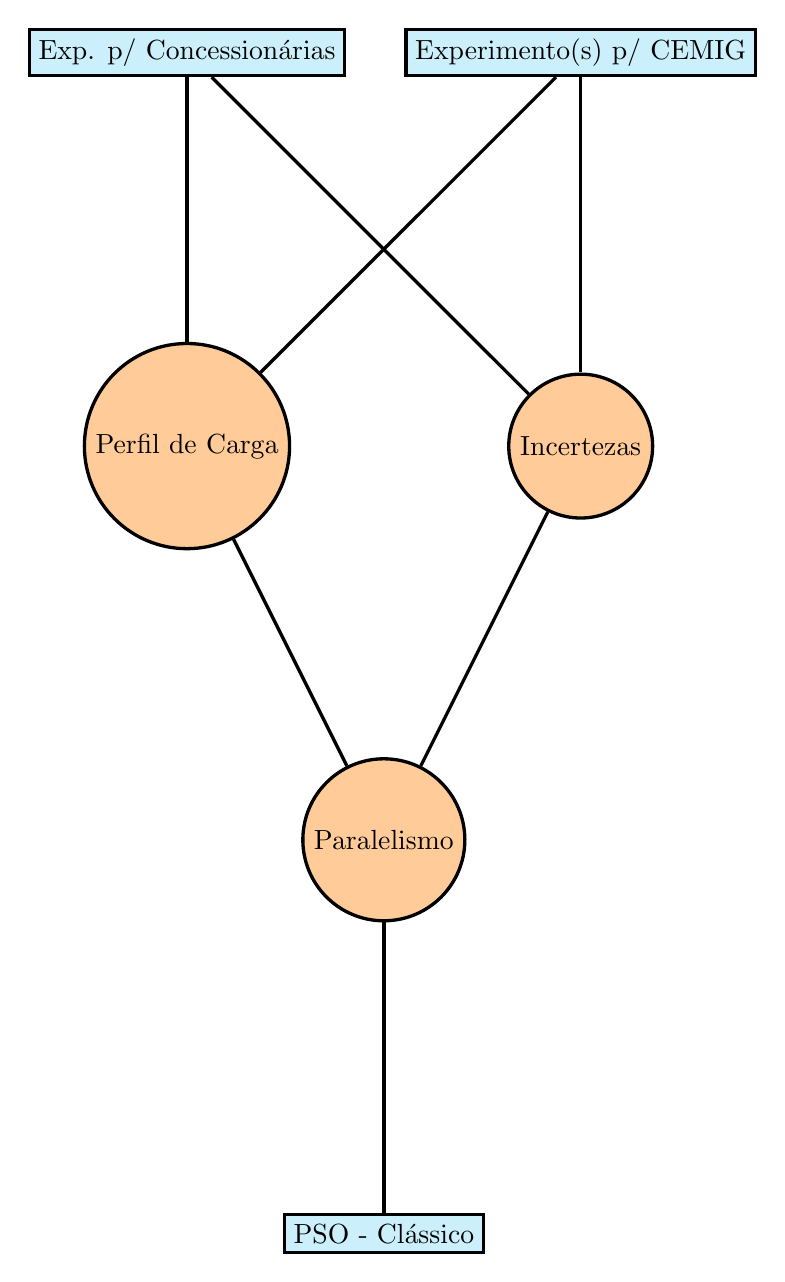
\begin{tikzpicture}
%% Draw system flow diagram
   \begin{scope}[xshift=-7.5cm,yshift=-5cm,very thick,
		node distance=5.0cm,on grid,>=stealth',
		block/.style={rectangle,draw,fill=cyan!20},
		comp/.style={circle,draw,fill=orange!40}]
   \node [block] (re)					{PSO - Clássico};
   \node [comp]	 (cb)	[above=of re]			{Paralelismo}  edge [-] (re);
   \node [comp]	 (ca1)	[above=of cb,xshift=-2.5cm]	{Perfil de Carga} edge [-] (cb);
   \node [comp]	 (ca2)	[right=of ca1]			    {Incertezas} edge [-] (cb);
   \node [block] (s1)	[above=of ca1]		{Exp. p/ Concessionárias} edge [-] (ca1) edge [-] (ca2);
   \node [block] (s2)	[right=of s1]		{Experimento(s) p/ CEMIG} edge [-] (ca2) edge [-] (ca1);
   \end{scope}
\end{tikzpicture}

\section{Motivação}
A maior preocupação neste início de trabalho é ser assertivo na escolha do problema. Apesar de reconhecer a importância de aprofundar na compreensão de ferramentas matemáticas utilizadas, percebe-se que é primordial focar no que é mais importante para o dia a dia das equipes de planejamento/operação em uma concessionária.

Percebe-se que o desejo dos engenheiros de planejamento e operação são processos simples e com alta capacidade de reprodutividade. Acredita-se que o cliente deste trabalho queira alcançar, com o mínimo de esforço, o objetivo final, que é a melhoria dos níveis de tensão. Sem grandes custos financeiros.

Pensando desta forma, gostaria de obter, como resultado deste trabalho, uma metodologia capaz de mapear com qualidade as formas ótimas de inserir potência reativa em um sistema, considerando qualquer nível de carregamento da rede.

%\section{Conclusão}
%By Luiz Le Roy et. al.: \cite{arruda2005calculation}, \cite{adriano2006modelos} e \cite{adriano2006efeitos}.

% Can use something like this to put references on a page
% by themselves when using endfloat and the captionsoff option.
\ifCLASSOPTIONcaptionsoff
  \newpage
\fi

\bibliographystyle{ieeetran}
\bibliography{bibliography}

\begin{IEEEbiographynophoto}{Luiz~Le~Roy}
é estudante do Programa de Pós-graduação em Engenharia Elétrica da Pontif\'icia Universidade Cat\'olica de Minas Gerais.
\end{IEEEbiographynophoto}

% that's all folks
\end{document}